\documentclass[12pt,twoside]{toptesi}
\usepackage{listings}
%\usepackage[latin9]{inputenc}
%\usepackage[italian]{babel}
\lstset{language=Java,breaklines=true,basicstyle=\footnotesize,frameround=fttt,frame=trBL}
\facolta[III]{Ingegneria}
\NomeMonografia{Relazione di progetto} 
\monografia{Automazione Discreta}
\corsodilaurea{Ingegneria Informatica} 
\candidato{Luca \textsc{Belluccini}\\
	Piergiuseppe \textsc{Bettassa Copet}\\
	Manuele \textsc{Bommarito}\\
	Matteo \textsc{Casalino}\\
	Davide \textsc{Ferri}\\
	Ivan \textsc{Lazzero}}
\sedutadilaurea{\textsc{Anno~accademico} 2008-2009}
\logosede{logopolito}
\includeonly{% 
	introduzione,%
	meccanica,%
	motori_sensori,%
	navigation, %
	checkers,%
	capitolo_roboCheckers,%
	teamwork,% 
	%capitolo3,% 
	%capitolo4% 
} 
\begin{document}\errorcontextlines=9
	\frontespizio
\indici
\sommario
Questo � il sommario
	\chapter{Meccanica del Robot}
Il robot � costituito da tre diverse parti funzionali: una base dotata di ruote motrici,
 un braccio rotante ed un sistema di leve a forbice.

\section{La base}
La base del robot � stata costruita partendo da un modello presente sul sito
della \emph{Lego}\textregistered 
(\emph{http://www.active-robots.com/products/mindstorms4schools/building-instructions/Build-RoboArm.pdf} Figura \ref{Base}) 
e modificato come segue: il motore B, che nello schema originale si occupava di far ruotare il braccio, continua nella sua funzione mentre il motore A
trasferisce la sua funzione da far muovere in avanti il braccio a gestire la trazione del robot.\\

\begin{figure}
	\begin{center}
		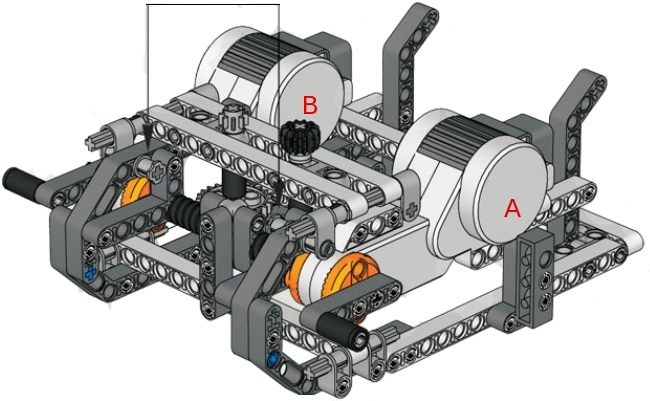
\includegraphics[scale=0.5]{img/base.png}
		\caption{Struttura iniziale della Base \label{Base}}
	\end{center}
\end{figure}

Per permettere al robot di avanzare, la base � stata montata su quattro ruote di
cui le due anteriori sono le ruote motrici. Quest'ultime sono collegate tra di
loro con un asse motore comune, che riceve il movimento tramite un gioco di
ingranaggi conici trasformando la rotazione dall'asse veticale, prodotta dal
motore A pi� la vite archimedea, in un movimento sull'asse orizzontale
necessario per l'avanzamento del robot.\\

Questo sistema ha per� mostrato delle carenze di precisione dovute da torsioni,
flessioni e giochi meccanici.\\

Per ovviare a ci� si � proceduto in pi� modi: 
\begin{itemize} 
  \item Creando un nuovo sistema di aggancio dell'albero motore verticale, in
 		 modo da minimizzarne la flessione. Nello specifico, si � inserita una
  		 piastrina triangolare per 'agganciare' l'albero motore, il pi� vicino
  		 possibile al punto di contatto tra gli ingranaggi conici. Figura
  		 \ref{ALBERO} FOTO ALBERO MOTORE 
  		 \begin{figure}
           \begin{center}
			 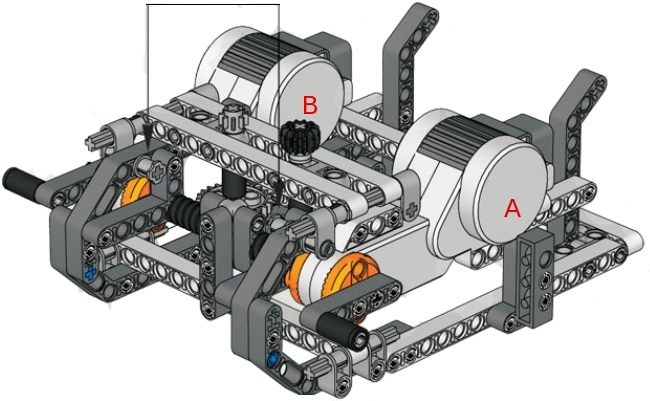
\includegraphics[scale=0.5]{img/base.png}
			 \caption{Struttura iniziale della Base \label{ALBERO}}
		   \end{center}		
		 \end{figure}
 
  \item Inserendo sotto la base un asse rigido che arrivi da ruota a ruota, in
  		 modo da ridurre la flessione dell'albero motore, dovuta al peso del robot
  		 stesso. \ref{SOSPENSIONI} FOTO SOSPENSIONI
 
		\begin{figure}
         \begin{center}
			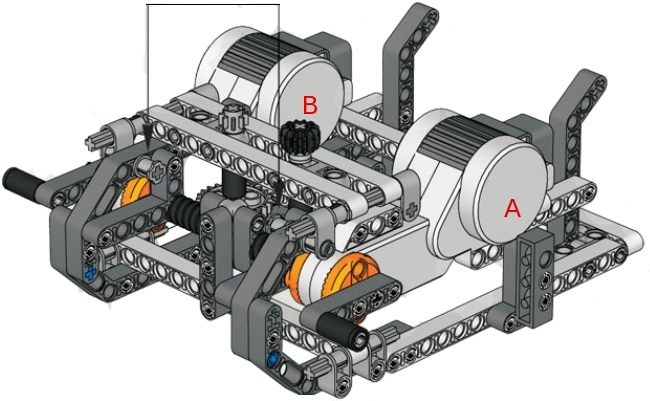
\includegraphics[scale=0.5]{img/base.png}
			\caption{Struttura iniziale della Base \label{SOSPENSIONI}}
		  \end{center}
		\end{figure} 

  \item Inserendo delle parti non non originali della 
  		\emph{Lego}\textregistered~per cercare di ridurre i giochi meccanici,
  		nello specifico si sono inserite delle rosette nella sede delle viti
  		achimedee e nei vari supporti degli assi. \ref{ROSETTE} FOTO ROSETTE
  		
  		\begin{figure}	
           \begin{center}	
			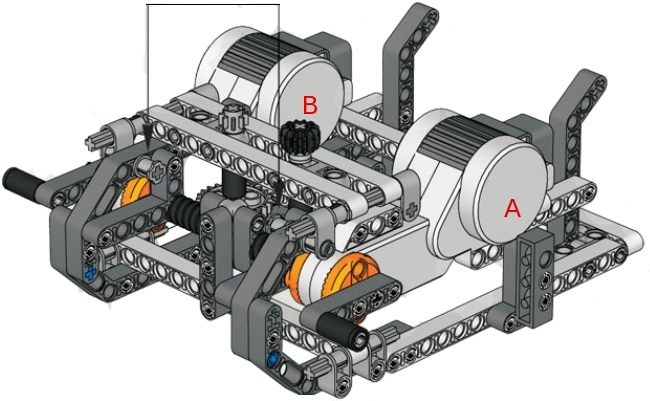
\includegraphics[scale=0.5]{img/base.png}
			\caption{Struttura iniziale della Base \label{ROSETTE}}
		  \end{center}			
		\end{figure}  	 


\end{itemize} 

Per i problemi relativi alle torsioni degli alberi non si � potuto fare nulla,
essendo questi problemi puramente dipendenti dalla natura fisica degli stessi e
non dal sistema di montaggio.

\section{Il Braccio}
Per la costrizione del braccio si � nuovamente presa ispirazione dalle
istruzioni della \emph{Lego}\textregistered~, modificandolo in modo da renderlo
rigido e non pi� snodabile Figura \ref{braccio} . Per effettuare questa
modifica si � elimitato il movimento centrale e fissati i montanti del braccio
tramite due 'traverse'.

  		\begin{figure}
          \begin{center}		
			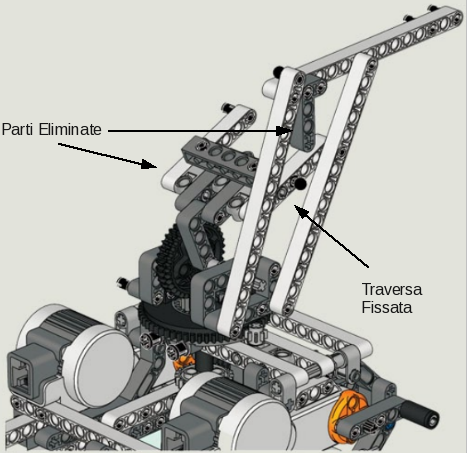
\includegraphics[scale=0.5]{img/braccio.png}
			\caption{Struttura del Braccio \label{braccio}}
		  \end{center}
		\end{figure} 

\section{Sistema di leve a forbice}
	\chapter{Motori e sensori}
In questo capitolo verranno esaminati in dettaglio
le API (\emph{Application Programming Interface}) 
utilizzate nella gestione dei motori e dei sensori.\\
Per brevit� di trattazione verrano illustrati solamente i
comandi pi� comuni e utilizzati, si rimanda alla 
documentazione di \emph{Lejos} per approfondimenti.

\section{Il motore}
Nei motori di \emph{Lego}\textregistered~NXT sono dotati di un
tachimetro che, con un controllo in retroazione,
permette di far ruotare i motori per un determinato angolo,
con un'incertezza di 2 gradi.\\
Al brick NXT � possibile collegare fino a tre motori.  

\subsection{La classe Motor}
La classe \texttt{Motor} consente sia il controllo diretto
di un motore collegato ad una porta (A,B,C), sia l'istanziamento
di un nuovo oggeto di tipo \texttt{Motor} tramite il costruttore.\\
La prima modalit� � implementata tramite campi statici dichiarati
nella classe, la seconda tramite il costruttore:
\begin{lstlisting}
	Motor(TachoMotorPort port)
\end{lstlisting}
che ha come parametro un'implementazione dell'interfaccia
\texttt{TachoMotorPort}, ad esempio \texttt{MotorPort}, che 
indichi a quale porta associare il nuovo oggetto.\\
\\
La classe \texttt{Motor} mette a disposizione numerosi metodi,
i pi� utilizzati sono:
\begin{lstlisting}
 /** rotazione continua all'indietro */
 void backward(); 
 /** rotazione continua in avanti */
 void forward();
 /** velocit� corrente in gradi al secondo */
 int getSpeed();
 /** restituisce vero se il motore � in movimento */
 boolean isMoving();   
 /** restituisce vero se il movimneto di rotazione ad 
  un angolo specifcio non � stato completato */
 boolean isRotating();
 /** azzera il contatore del tachimetro */
 void resetTachoCount();
 /** inverte il senso di rotazione */
 void reverseDirection();
 /** ruota di un determinato angolo rispetto alla  posizione 
	 corrente, se  immediateReturn � true, allora il metodo non 
	 � bloccante e resituisce subito il controllo completando 
	 la rotazione autonomamente */
 void rotate(int angle, boolean immediateReturn);  
 /** ruota all'angolo limitAngle rispetto al riferimento, 
	 se  immediateReturn �  true, allora il metodo non � 
	 bloccante e resituisce subito  il controllo completando 
	 la rotazione autonomamente */
 void rotateTo(int limitAngle, boolean immediateReturn);
 /* imposta la potenza del motore, power <= 900 */
 void setPower(int power);
 /* ferma il motore */
 void stop(); 
\end{lstlisting}

\section{I sensori}
Al brick \emph{Lego}\textregistered~NXT � possibile
collegare diversi tipi di sensori.\\
I sensori prodotti dalla casa madre \emph{Lego}\textregistered~sono:
\begin{itemize}
  \item pressione
  \item luce
  \item suono
  \item colore
  \item ultasuoni
  \item bussola
  \item accelerometro
  \item infrarossi
  \item giroscopio
\end{itemize} 
Molti altri tipi di sensori, prodotti da ditte specializzate o da 
appassionati, possono essere acquistati on-line.\\
\\
Il brick \emph{Lego}\textregistered~NXT supporta fino a 4 sensori.\\
La classe \texttt{SensorPort} mette a disposizione 4 campi statici
(S1, S2, S3 ed S4), che sono istanze di \texttt{SensorPort} 
e che coincidono alle 4 porte del bick.\\
Siccome i dati letti hanno significato diverso per ogni tipo di
sensore, per ciascuno di essi \emph{Lejos} fornisce
una classe in grado di interpretare corretamente i dati ricevuti.

\subsection{Il sensore di pressione}




\subsection{Il sensore di colore}

	\chapter{Il package Navigation}
Il \emph{package} \texttt{it.polito.Navigation} contiene le classi deputate a gestire i movimenti del Robot sulla scacchiera.\\
In particolare sono stati progettati due controllori: \texttt{CheckersNavigator} e\\ \texttt{ArmController} che sono responsabili rispettivamente della navigazione nelle due direzioni orizzontali e in quella verticale.\\
Di seguito si entrer� nel dettaglio delle implementazioni delle classi sopra
citate e dei relativi helper.
\section{La classe LashMotor}
I motori del NXT dispongono di un tachimetro incorporato, pertanto le API di
\emph{Lejos} mettono a disposizione una classe \texttt{Motor} che consente di
controllarli con una buona precisione. In particolare, mediante i metodi
\texttt{rotate()} e \texttt{rotateTo()}, � possibile ruotare il rotore di un
angolo arbitrario con un'incertezza di pi� o meno 2 gradi.\\
Per come sono stati impiegati i motori, tuttavia, si sono determinati dei giochi
meccanici non trascurabili tra il movimento dei rotori e lo spostamento effettivo
del Robot sulla scacchiera, che avrebbero causato errori di
posizionamento superiori alla lunghezza di mezza casella.\\
La classe \texttt{LashMotor} estende l'API \texttt{Motor} di \emph{Lejos} e
rappresenta un motore in grado di recuperare un gioco costante (che deve quindi
essere preventivamente stimato\footnote{La stima dei giochi � stata effettuata
empiricamente cercando di determinare l'angolo minimo tale da indurre un
movimento del Robot, in seguito a un cambio di verso di rotazione.}) in modo
trasparente all'utilizzatore.\\
Il metodo reimplementato in \texttt{LashMotor} � \texttt{rotateTo()}: il recupero
del gioco avviene solo quando si verifica un'inversione (si � scelto il verso
negativo perch� si richiede che i motori vengano inizializzati con gioco nullo
nel verso positivo, ad esempio a fine calibrazione) semplicemente
decrementando l'angolo di destinazione della costante \texttt{lash} stimata.\\
\begin{lstlisting}
	public void rotateTo(int limitAngle, boolean nonBlocking) {
		if (limitAngle < super.getTachoCount())
			limitAngle -= lash;
		super.rotateTo(limitAngle, nonBlocking);
	}
\end{lstlisting}
Si noti che, nel caso di cambio di direzione inverso, il recupero avviene senza
bisogno di modificare l'angolo di destinazione infatti, detti $c$ la costante
\texttt{lash} e $\theta_0$ l'angolo di partenza si avrebbe:
\begin{figure}[htbp]
	\begin{center}
		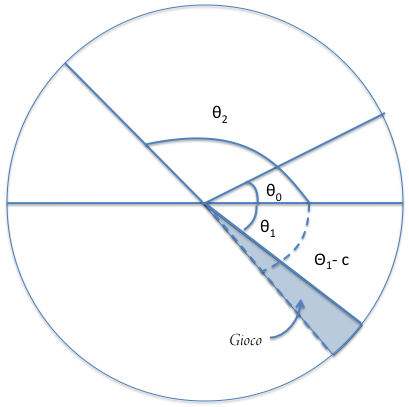
\includegraphics[scale=0.7]{img/lashMotor.png}
		\caption{Recupero dei giochi in un motore LashMotor \label{lashMotor}}
	\end{center}
\end{figure} 
\itemize
\item Rotazione all'angolo $\theta_1 < \theta_0$
	$$\theta = \theta_0 + (\theta_1 - \theta_0 - c) = \theta_1 - c$$
\item Rotazione all'angolo $\theta_2 > \theta_1$
	$$\theta = \theta_1 - c + (\theta_2 - (\theta_1 - c)) = \theta_2$$

\section{L'interfaccia  CheckersNavigator}
Questa interfaccia astrae le funzionalit� di movimento bidimensionale sulla scacchiera 8x8; i metodi pi� importanti sono:

\begin{lstlisting}
/** Ritorna la posizione X [0; 7] */
public int getX(); 
/** Ritorna la posizione Y [0; 7] */
public int getY(); 
/** Muove il braccio sulla casella (X, Y) */
public void goTo(int newX, int newY) throws NotCalibratedException; 
/** Muove il braccio sulla casella "base" */
public void goHome() throws NotCalibratedException; 
/** Modifica la velocit� dei motori */
public void setSpeed(int speedA, int speedB);
/** Effettua la calibrazione */
public void calibrate();
\end{lstlisting}
Si noti come i metodi che comportano un movimento non possano essere eseguiti se prima non � stata effettuata la calibrazione (eccezione \texttt{NotCalibrated\-Exception}).\\
Esamineremo ora le implementazioni che sono state progettate per questa interfaccia.

\subsection{La classe SimpleNavigator}
Questa prima implementazione si basa su un mapping statico di tutte le caselle relativo ad un punto iniziale su cui il Robot tenta di posizionarsi in fase di calibrazione.

\subsubsection{Calibrazione}
Il Robot, per come � costruito, pu� ruotare il suo braccio agendo sul motore B, o
pu� spostarlo avanti e indietro agendo sul motore A.\\ Il primo metodo di
calibrazione che � stato pensato, � pertanto semplicemente mirato a portare il
braccio in una posizione nota (punto rosso in Figura \ref{simpleNavigatorGrid}),
in modo da poter usare offset predeterminati (relativi ad essa) per spostarlo su
tutte le altre caselle. \\ \begin{figure}[ht]
\begin{center}
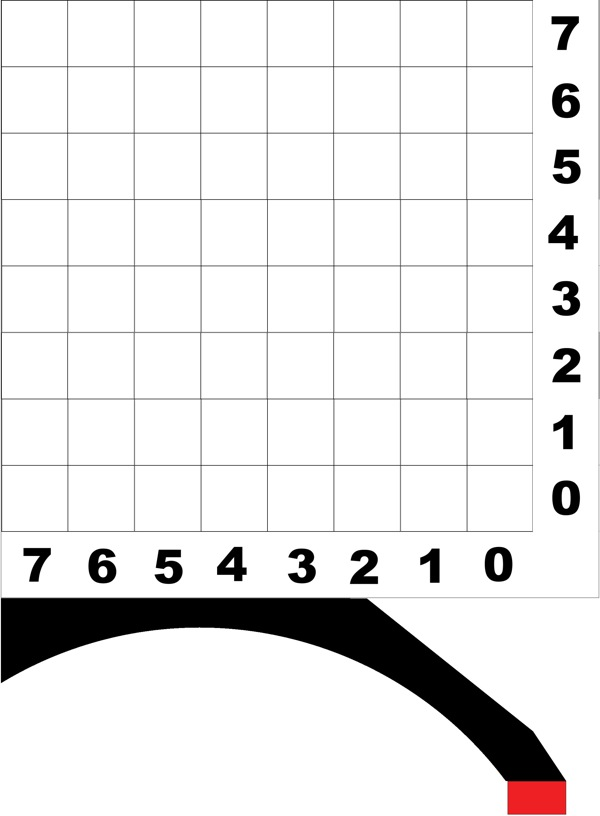
\includegraphics{img/simpleNavigatorGrid.jpg}
\caption{Scacchiera SimpleNavigator \label{simpleNavigatorGrid}}
\end{center}
\end{figure}
Il metodo \texttt{calibrate()} non fa altro che ruotare il braccio verso destra finch� il sensore di colore montato su di esso non rileva il colore rosso, a quel punto recupera eventuali giochi dei motori e azzera i contatori di distanza angolare in essi contenuti.

\subsubsection{Navigazione}
Gli angoli di destinazione cui vengono fatti ruotare i motori sono calcolati semplicemente come\footnote{X e Y sono rispettivamente le  coordinate di ascissa e di ordinata delle caselle}: 
\begin{lstlisting}
destAngleA = offA+posy[newY]+dely[newX];
destAngleB = offB+posx[newX];
\end{lstlisting}
I vettori \texttt{posx} e \texttt{posy} definiscono l'offset in funzione delle rispettive coordinate;
il vettore \texttt{dely} contiene le correzioni da effettuare sull'asse y in funzione della coordinata x,
in modo da recuperare gli scostamenti in verticale dati dal fatto che il braccio si muove su un arco
di circonferenza.\\
Le costanti \texttt{offA} e \texttt{offB} definiscono invece l'offset necessario a portare il braccio
sulla casella (5,0) che costituiva il punto pi� comodo cui riferire la taratura di tutte le altre caselle.

\subsection{La classe MathNavigator}
Il limite pi� evidente del \texttt{SimpleNavigator} � dato dai vincoli statici di allineamento
che devono sussistere tra Robot e scacchiera. \'E chiaro infatti che, qualora non si
posizionasse il braccio in modo da far coincidere il suo centro di rotazione con il centro del
tratto di circonferenza in Figura \ref{simpleNavigatorGrid}, questo non riuscirebbe a seguire l'arco stesso
in fase di calibrazione e non potrebbe quindi successivamente posizionarsi sulla scacchiera.\\
Per ovviare a questo fatto � stato introdotto un modello geometrico del sistema, in modo da avere a
disposizione una soluzione analitica del problema.\\
Di nuovo andremo ad illustrare separatamente le fasi di calibrazione e di navigazione che, in questo caso,
risultano ovviamente pi� complesse.
\subsubsection{Calibrazione}
La costruzione cui si far� riferimento nel seguito � quella in Figura \ref{mathNavigator1}, in cui si possono
osservare la scacchiera quadrata di lato $l$ e la circonferenza di centro $C$ e raggio $r$ descritta dal braccio
che si muove su di essa.\\
\begin{figure}[ht]
\begin{center}
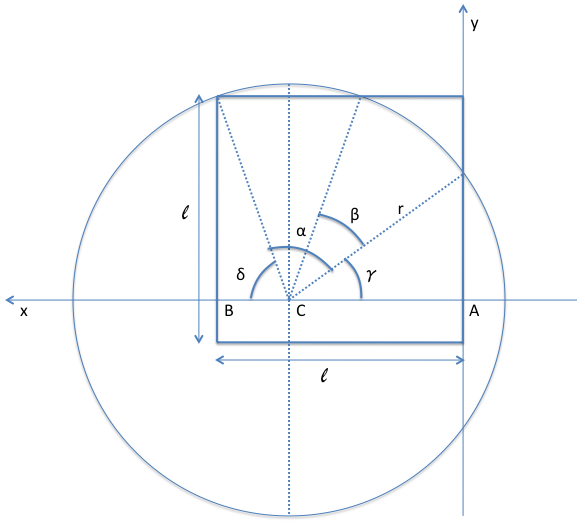
\includegraphics[scale=0.65]{img/mathNavigator1.png}
\caption{MathNavigator, calibrazione \label{mathNavigator1}}
\end{center}
\end{figure}
L'idea � quella di permettere al Robot di determinare il rapporto $\frac{\overline{BC}}{\overline{CA}}$
(e quindi la posizione del suo centro rispetto alla scacchiera) a partire dalla misura, eseguita in fase di
calibrazione mediante i sensori disponibili, di parametri geometrici.\\
Il parametro pi� comodo da misurare, semplicemente usando il sensore di colore e il tachimetro interno ai motori,
� quello che in Figura \ref{mathNavigator1} � indicato come angolo $\alpha$, cio� l'angolo descritto dal braccio
quando sorvola l'intera scacchiera. Una volta determinato $\alpha$ e
ipotizzando $\overline{BC}<\overline{CA}$ si pu� risolvere il problema in forma chiusa:
$$\delta = \frac{\pi - \alpha + \beta}{2}$$
$$\gamma = \delta - \beta$$
\begin{center}
\begin{math}
l = r\left(\cos\gamma+\cos\delta\right) =
r\left(\cos\left(\frac{\pi-\alpha+\beta}{2}\right)+
\cos\left(\frac{\pi-\alpha+\beta}{2}-\beta\right)\right)=
r \left(\cos\left(\frac{\pi-\alpha}{2}\right)\cos\left(\frac{\beta}{2}\right)-
\sin\left(\frac{\pi-\alpha}{2}\right)\sin\left(\frac{\beta}{2}\right) +
\cos\left(\frac{\pi-\alpha}{2}\right)\cos\left(\frac{\beta}{2}\right) +
\sin\left(\frac{\pi-\alpha}{2}\right)\sin\left(\frac{\beta}{2}\right)\right) =
2r\cos\left(\frac{\pi-\alpha}{2}\right)\cos\frac{\beta}{2}
\end{math}
\end{center}
e quindi:
$$\beta = 2\arccos\left(\frac{l}{2r\cos\left(\frac{\pi-\alpha}{2}\right)}\right)  = 2\arccos\left(\frac{l}{2r\sin\frac{\alpha}{2}}\right)$$
$$\overline{CA} =  r\sin\left(\frac{\alpha+\beta}{2}\right)$$ 
Le relazioni appena ricavate evidenziano immediatamente che l'accuratezza della stima del rapporto
$\frac{l}{r}$ � un parametro critico. Pi� avanti si discuteranno le problematiche correlate a questo punto.\\
\begin{figure}[ht]
\begin{center}
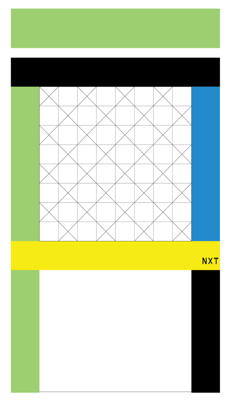
\includegraphics[scale=0.7]{img/mathNavigatorGrid.png}
\caption{Scacchiera MathNavigator \label{mathNavigatorGrid}}
\end{center}
\end{figure}
La fase di calibrazione consiste quindi essenzialmente nell'eseguire la stima dell'angolo $\alpha$, perci�
la scacchiera � stata ridisegnata come in Figura \ref{mathNavigatorGrid}.
Il Robot deve essere posizionato tra le bande verticali verde e nera, con
l'unico vincolo che la direzione del suo movimento in avanti/indietro sia parallela all'asse $y$ della scacchiera.\\
Per misurare $\alpha$ il braccio ruota verso sinistra fino a raggiungere la
banda verde, successivamente viene azzerato il contatore angolare del motore B e
si ruota nel senso opposto finch� non � stata raggiunta la banda nera. A questo punto il Robot determina la sua posizione rispetto alla scacchiera e avanza fino alla banda blu
(angolo in basso a destra della scacchiera).\\
Chiaramente il rapporto (\texttt{coeffB}) tra la distanza angolare misurata dal contatore interno al motore e
l'effettivo valore di $\alpha$ in radianti � un altro parametro che � necessario conoscere con sufficiente
precisione, come anche l'analoga costante per il motore A (\texttt{coeffA}).

\subsubsection{Navigazione}
Per navigare verso una posizione qualsiasi sulla scacchiera, a questo punto, � sufficiente effettuare il
cambio di coordinate $(\theta, C_y)=\mathcal{F}(P_x,P_y)$
\begin{figure}[ht]
\begin{center}
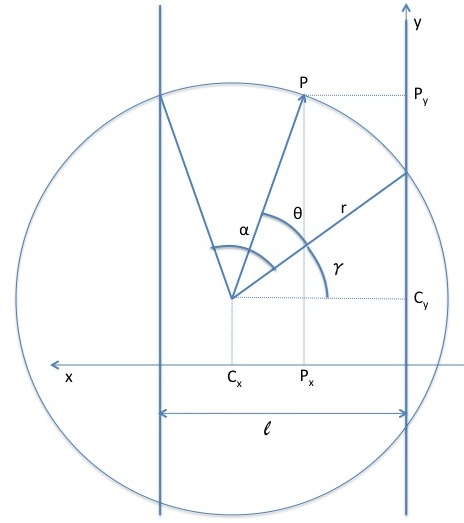
\includegraphics[scale=0.7]{img/mathNavigator2.png}
\caption{MathNavigator, navigazione \label{mathNavigator2}}
\end{center}
\end{figure}
dove $(P_x,P_y)$ sono le coordinate della destinazione, $(\theta,C_y)$ i comandi da fornire ai motori
B e A (opportunamente riscalati per \texttt{coeffB} e \texttt{coeffA}) e
$$\mathcal{F}:\bigg \{
\begin{array}{l}
\theta = \arccos\left(\frac{C_x-P_x}{r}\right) - \gamma \\
C_y = P_y - r\sin\left(\arccos\left(\frac{C_x-P_x}{r}\right)\right)
\end{array}
$$
con
$$\gamma = \frac{\pi-\alpha-\beta}{2}$$
$$C_x = r\sin\left(\frac{\alpha+\beta}{2}\right)$$
Il cambio di coordinate viene eseguito dal metodo \texttt{moveTo()}, mentre \texttt{goTo()} si occupa soltanto
di offrire compatibilit� verso l'interfaccia (che impone una casella di destinazione) passando a \texttt{moveTo()}
le coordinate di destinazione espresse in centimetri.

\subsubsection{Stima dei parametri ed effetto delle incertezze}
\'E gi� stato evidenziato come, al fine di ottenere un posizionamento soddisfacente, sia necessario disporre di una
stima sufficientemente precisa delle costanti che compaiono nelle equazioni che sono state presentate.\\
Intendiamo di seguito dare un'idea dei ragionamenti che sono stati fatti per ricavarle e dei limiti del modello
matematico ricavato.
\paragraph{Stima di \texttt{coeffA} e \texttt{coeffB}}
\begin{figure}[ht]
\begin{center}
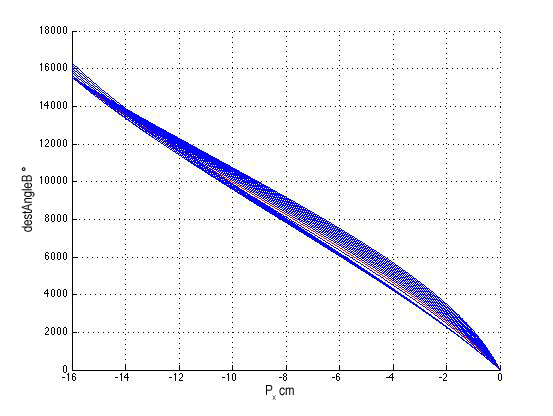
\includegraphics[scale=0.6]{img/theta(CoeffB).png}
\caption{Comando motore B in funzione di $P_x$, al variare di coeffB\label{theta(CoeffB)}}
\end{center}
\end{figure}
\begin{figure}[ht]
\begin{center}
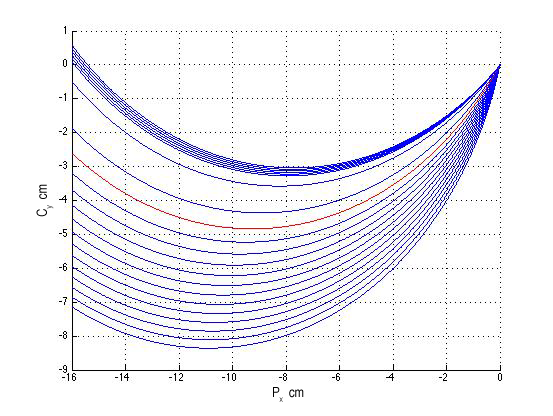
\includegraphics[scale=0.6]{img/Cy(CoeffB).png}
\caption{$C_y$ in funzione di $P_x$, al variare di coeffB\label{Cy(CoeffB)}}
\end{center}
\end{figure} 
Per ricavare il legame che sussiste tra la rotazione dei rotori e la distanza o gli angoli effettivamente coperti
dal movimento del braccio, si � pensato di misurare distanze (tacche parallele distanziate di 2 cm) e angoli
(si � scelto l'angolo piatto per ridurre i problemi di allineamento rispetto al centro) noti, mediando i
risultati ottenuti.\\
Un ulteriore raffinamento delle stime ottenute � stato possibile grazie al confronto del movimento del braccio, con
il plot dell'andamento delle coordinate $(\theta,C_y)$ al variare di \texttt{coeffB} (Figure \ref{theta(CoeffB)} e \ref{Cy(CoeffB)})
\paragraph{Rapporto $\frac{l}{r}$}
La lunghezza $l$ del lato della scacchiera � nota senza problemi ed � pari a 16 cm. Un discorso diverso dev'essere
fatto per il raggio del braccio $r$ che, per ragioni meccaniche, dipende in modo non trascurabile da $\theta$.
Infatti, al variare di $\theta$, il centro del sensore di colore montato sul braccio descrive pi� precisamente un
ellisse, che nel modello presentato � invece stato approssimato ad una circonferenza.\\
La stima del raggio � pertanto soggetta ad un'incertezza superiore al 4\%, $r=12\pm0.5$ cm e l'errore finale
che ne deriva dipende dalla posizione iniziale del Robot (perch� cambiano i parametri dell'ellisse) arrivando a
superare la lunghezza di una casella.\\
Il problema � stato risolto aggiungendo una fase di \emph{post-calibrazione} (metodo \texttt{calibrateY()}) durante
la quale il Robot si porta sulla fascia bianca ricavata in cima alla scacchiera
(Figura \ref{mathNavigatorGrid}) e, muovendosi a passi discreti di 2 cm (larghezza di una casella), costruisce un vettore di offset che contiene le
correzioni da apportare lungo y alla sua posizione. Questo vettore viene poi usato per correggere ogni successivo
posizionamento.

\section{La classe ArmController}
Questa classe controlla il movimento verticale del pantografo montato sul braccio. Per farlo, si serve del motore C
posizionato sul braccio stesso e del sensore di pressione.\\
Il pantografo � montato in modo che, quando � chiuso (braccio in alto), una delle leve agisca sul sensore di
pressione. Perci� il metodo \texttt{up()} non fa altro che muovere il motore finch� non viene rilevata una pressione
sul sensore.\\
Il metodo \texttt{down()} invece ruota il motore di un angolo che � stato determinato in modo da portare il
pantografo alla sua massima estensione (braccio in basso).\\
Al fine di rendere i movimenti del braccio pi� rapidi, si � manifestata la
necessit� di poter eseguire le chiamate ai metodi \texttt{up()} e
\texttt{down()} in modo non bloccante, ad esempio:
\begin{lstlisting}
arm.up(true); // non bloccante
navigator.goTo(nextMove.getLastTo()); // il braccio si alza e contemporanemente si posiziona sulla casella di destinazione
\end{lstlisting}
Implementare questo tipo di comportamento � banale per il metodo
\texttt{down()}, perch� questo esegue al suo interno una chiamata al metodo
\texttt{Motor.rotateTo()} che le API di Lejos gi� prevedono in versione non 
bloccante.
\begin{lstlisting}
public void down(boolean immediateReturn) {
	if (state == DOWN || state == GODOWN)
		return;
	// wait for stop
	while (state != UP)
		Thread.yield();
	synchronized (armRegulator) {
		state = GODOWN;
	}
	MC.rotateTo(goDownRounds,immediateReturn);
}
\end{lstlisting}
Un discorso diverso deve essere fatto per il metodo \texttt{up()}. In questo
caso � necessario disporre di un meccanismo che controlli periodicamente lo
stato del sensore di pressione e fermi il motore al momento giusto, anche se
\texttt{up()} � gi� ritornato.\\
A questo scopo � stata progettata la classe innestata \texttt{ArmRegulator}:
\begin{lstlisting}
public class ArmRegulator extends Thread {
   public void run() {
     while (true) {
        synchronized (this) {
           switch (state) {
              case GOUP:
                 if (TS.isPressed()) {
                    MC.stop();
                    MC.resetTachoCount();
                    state = UP;
                 } break;
              case GODOWN:
                 if (!MC.isMoving()) state = DOWN;
                 break;
              } // end switch
           } // end synchronized
           try {sleep(1);} catch(InterruptedException ie ) {}
        } // end while } }
\end{lstlisting}
Un oggetto di tipo \texttt{ArmRegulator} viene istanziato ed eseguito in un
thread autonomo, al momento della creazione dell'\texttt{ArmController}:
\begin{lstlisting}
private ArmController (Motor MC, TouchSensor TS) {
	this.MC = MC;
	this.TS = TS;
	this.armRegulator.setDaemon(true);
	this.armRegulator.start();
}
\end{lstlisting}
A questo punto il metodo \texttt{up()} non deve fare altro che aggiornare lo
stato del sistema a \texttt{GOUP}, del resto si occuper� \texttt{armRegulator}:
\begin{lstlisting}
public void up(boolean immediateReturn) {
	if (state == UP || state == GOUP)
		return;
	// wait for stop
	while (state != DOWN)
		Thread.yield();
	synchronized (armRegulator) {
		if (!TS.isPressed()) {
			state = GOUP;
			MC.forward();
		} else {
			state = UP;
		}
	}
	if (immediateReturn)
		return;
	while (MC.isMoving()) //should be equivalent to (state != UP) but maybe more secure
		Thread.yield();
}
\end{lstlisting} 
	\chapter{Il package Checkers}
Il \emph{package} \texttt{it.polito.Checkers} racchiude un insieme di
classi in grado di gestire una partita a Dama.\\ 
Il motore del gioco � racchiuso nella classe \texttt{Engine}, mentre le altre
classi fungono da interfaccia verso il resto del progetto.\\
Il motivo di questa organizzazione � dato dal fatto che tutti i metodi di
\texttt{Engine} provengono da una Java applet sviluppata da un gruppo di studenti
del \emph{California Institute of Technology} (http://www.cs.caltech.edu).
Essendo questo codice poco orientato ad oggetti e per la quasi totalit�
costituito da metodi statici, � stato racchiuso in una sola classe i cui metodi
vengono richiamati dagli oggetti \emph{wrapper} che la circondano.\\
la scelta di impiegare codice gi� pronto in questa parte � stata
mutuata essenzialmente dai limiti temporali (anche se non nascondiamo che in pi�
occasioni avremmo preferito riscriverlo da zero!) nonch� dal fatto che
implementare l'intera intelligenza per il gioco della dama avrebbe esulato dalla
natura del progetto stesso.
\section{Engine}
Il cuore della classe � costituito dai metodi \texttt{MiniMax()},
\texttt{Evaluate()} e \texttt{generate\\\_moves()}. Tutti gli altri metodi
servono a fornire supporto a questi tre.\\
Tra essi \texttt{generate\_moves()} � quello pi� complicato, perch� si occupa di
creare il vettore delle mosse possibili per un determinato giocatore, data una
qualsiasi configurazione (purch� valida) delle pedine sulla scacchiera.
Pertanto si serve di una serie di altre funzioni che, sostanzialmente,
determinano quali mosse, tra tutte quelle possibili, sono effettivamente valide
secondo le regole della Dama.
\subsection{MiniMax}
Nella teoria dei giochi un algoritmo si definisce di tipo \emph{MiniMax}, se �
finalizzato a \emph{mini}mizzare la \emph{massima} perdita possibile.\\
In un gioco a turni, come la Dama, l'algoritmo si esprime in modo ricorsivo
come segue:
\lstset{tabsize=2}
\begin{lstlisting}
function minimax(node, depth)
	IF is_terminal(node) OR depth = 0
		return Evaluate(Nodo)
	IF turn = opponent
		alpha := +inf
		FOREACH child of node
			alpha := min(alpha, minimax(child, depth-1))
	ELSE {our turn}
		alpha := -inf
		FOREACH child of node
			alpha := max(alpha, minimax(child, depth-1))
	return alpha
\end{lstlisting}
Dato l'albero delle mosse possibili e data una profondit� massima di
ricorsione, si simula l'esecuzione della mossa che minimizza il valore della
migliore posizione raggiungibile dall'altro giocatore. Quindi l'algoritmo assegna
un valore ad ogni mossa legale, proporzionale a quanto essa diminuisce il valore della
posizione per l'altro giocatore.\\
La funzione \texttt{Evaluate} � fondamentale per valutare, ad ogni passo, la
bont� di quel determinato stato del gioco (i.e. quanto sia desiderabile per il
dato giocatore raggiungere quella posizione). Se un nodo � terminale (mossa
vincente) \texttt{MiniMax} deve ritornare $\pm\infty$ a seconda che il
turno corrente sia rispettivamente del primo o del secondo giocatore.
Altrimenti significa che si � raggiunto il limite di profondit� prefissato. In questo caso
\texttt{Evaluate} effettuer� una stima delle pedine in gioco assegnando un peso
ad ognuna di esse in funzione della loro posizione e del loro valore (ad
esempio, una dama vale di pi� di una normale pedina).\\
Ovviamente, se si fissasse una profondit� di ricorsione pari a infinito, non
sarebbe necessaria la stima euristica data da \texttt{Evaluate} e si
determinerebbe ad ogni passo una mossa ottima; � altrettanto chiaro tuttavia che
questa strategia � applicabile unicamente in giochi estremamente banali (ad
esempio il Tris), in quanto il numero di nodi da valutare cresce
esponenzialmente con la profondit� di ricerca ed � pari\footnote{Pi�
precisamente il \texttt{MiniMax} incluso nel progetto � ottimizzato mediante
potatura alpha-beta dell'albero delle decisioni (si rimanda a letteratura
specifica per eventuali approfondimenti) che riduce la complessit� a
$O\left(\sqrt{\overline{m}^d}\right)$ nel caso migliore} a $O(\overline{m}^d)$
(dove $\overline{m}$ � il numero medio di mosse possibili e $d$ � la profondit�)
determinando una complessit� finale di tipo NP completo.

\section{Square}
Rappresenta una casella sulla scacchiera. Mantiene semplicemente due attributi
interi che rappresentano le coordinate della casella.\\
I metodi contenuti in \texttt{Engine} non usano questo tipo di astrazione, ma
tipicamente mantengono separate le coordinate; la conversione in oggetti
\texttt{Square} viene eseguita dalle classi \texttt{Move} e \texttt{Board}

\section{Move e MoveCollection}
Le classi Move e MoveCollection sono state implementate per permettere una
gestione orientata agli oggetti delle mosse restituite dalla classe 
\texttt{Engine}.

\paragraph{Classe Move} 
Si occupa principalmente di rimappare a livello di oggetto la
singola mossa generata dalla classe \texttt{Engine}, questa astrazione viene
implementata dai metodi \texttt{toArray()}, che fa il mapping da oggetto a
vettore di interi, e \texttt{fromArray()}, che si occupa di convertire le mosse
da vettore ad oggetto.\\
La classe \texttt{Move} mantiene l'informazione sulle mosse in un attributo di
tipo \texttt{Square} contenente la casella di partenza, e in un vettore di
\texttt{Square} contenente tutte le destinazioni (in caso di prese
multiple vi sono memorizzati tutti i salti intermedi).

\paragraph{Classe MoveCollection} 
Rappresenta l'albero di tutte le destinazioni raggiungibili da una casella.
Viene utilizzata durante il controllo delle mosse fatte da \texttt{HumanPlayer}.

\section{Board}
\'E la rappresentazione della scacchiera all'interno del bricco. La classe
contiene, oltre alla posione attuale delle pedine, una collezione di
\texttt{MoveCollection} in cui sono incluse tutte le possibili mosse effettuabili dall'avversario.
Queste possono essere prelevate con il metodo \texttt{getPossibleMoves()} che
le restituisce sotto forma di \texttt{Vector<MovesCollections>}, oppure, se si necessita delle caselle di
partenza e di arrivo separatamente, sono disponibili i metodi
\texttt{getPossibleMoveFrom()} e \texttt{getPossibleMoveTo()}.\\
Quando si esegue una chiamata a \texttt{getPossibleMoves()}, il vettore
delle mosse possibili viene memorizzato in un attributo interno a
\texttt{Board}. In questo modo il vettore pu� essere scandito implicitamente
mediante il metodo \texttt{getPossibleMoveFrom()}, che restituisce una per
volta, ad ogni chiamata, le caselle di partenza delle mosse possibili.\\
L'indice relativo all'ultima casella restituita da
\texttt{getPossibleMoveFrom()} viene anch'esso memorizzato in un attributo di
\texttt{Board}, per cui - una volta individuata la casella di partenza - si pu�
procedere in modo analogo alla scansione delle possibili caselle di
destinazione, servendosi del metodo \texttt{getPossibleMoveTo()}.\\
L'ordine con cui viene scandito il vettore delle mosse possibili, dipende dal
lato della scacchiera su cui si trovava il braccio all'inizio della scansione.
Questo al fine di velocizzare l'intera esecuzione del processo.



	\chapter{Il package roboCheckers}
Il \emph{package} \texttt{it.polito.roboCheckers} contiene le classi per la gestione della partita e dei giocatori.\\
Sono presenti un'interfaccia Player successivamente implementata in \texttt{Human\-Player} e \texttt{ComputerPlayer} e la classe \texttt{Game} che effettua la partita vera e propria.

\section{L'interfaccia Player}
Questa interfaccia � usata per uniformare il giocatore robotico, il quale deve pensare ed effettuare la mossa, con il giocatore umano, di cui, invece, deve capirne la mossa effettuata. \\
Il metodo che esegue tutto questo �:
\begin{lstlisting}
/** Ritorna la mossa effettuata dal giocatore */
Move makeMove(final Board board) throws CantMoveException, IllegalMoveException, NotCalibratedException;
\end{lstlisting}
Come si pu� notare dalle eccezioni lanciabili, il metodo permette di riconoscere il caso in cui non ci siano pi� mosse disponibili sia da parte del robot che dell'umano e il caso in cui venga fatta una mossa non valida da parte dell'umano. Ovviamente tutto ci� non pu� funzionare se non � prima avvenuta la calibrazione (NotCalibratedException).

\subsection{ComputerPlayer}
Il suo metodo principale (\texttt{makeMove()}) si pu� sostanzialmente suddividere in due parti. Inizialmente viene scelta tra le mosse disponibili quella che permetter� di ottenere il punteggio migliore, attraverso il metodo \texttt{MiniMax()} della classe \texttt{Engine}. Successivamente la mossa viene mostrata, indicando con il braccio mobile prima la pedina che si vuole spostare e poi la casella in cui � stato scelto di spostarla, questo utilizzando le classi \texttt{CheckersNavigator} e \texttt{ArmController}.\\
Il livello di intelligenza della macchina � gestito mediante il livello di profondit� massimo della ricorsione, eseguita in \texttt{MiniMax()}, e viene impostato attraverso l'attributo \texttt{depth}.

\subsection{HumanPlayer}
Questa classe si differenzia dalla precedente in quanto il suo compito � riconoscere (e non pensare) la mossa fatta dal giocatore. La ricerca avviene analizzando tutte le possibili mosse. Per ogni mossa si controlla se la posizione di partenza � libera o ancora occupata dalla pedina. Nel caso sia occupata si passa a controllare la mossa successiva, altrimenti significa che si � trovata la pedina che � stata mossa. A questo punto si ricerca la posizione in cui � stata spostata la pedina, solo tra le destinazioni realmente possibili. Se viene riconosciuta una mossa valida, questa viene ritornata al metodo chiamante, altrimenti si lancia l'eccezione \texttt{IllegalMoveException}.

\section{Robot}
Contiene principalmente il metodo \texttt{main()} in cui si inizializzano i due
giocatori, di tipo ComputerPlayer o HumanPlayer, si fa eseguire la
calibrazione, si crea e si fa partire il gioco e si decreta il vincitore.
Questa classe istanzia anche il sensore di colore, il controllore del braccio
mobile, il \texttt{CheckersNavigator} e uno \texttt{HumanInput}\footnote{Vedi
sezione Factory} usato per l'interazione con il giocatore umano.

\section{Game}
Il metodo fondamentale di questa classe � sicuramente il metodo:
\begin{lstlisting}
public int play() throws NotCalibratedException
\end{lstlisting}
dove � gestita l'intera partita: sia l'alternarsi dei turni tra i due giocatori, sia l'aggiornamento della scacchiera virtuale memorizzata nella macchina.
\'E strutturato in un ciclo do-while che continua fino alla vittoria di uno dei giocatori. Al suo interno si controlla se il giocatore ha ancora una mossa disponibile e se l'ha effettuata correttamente, attraverso il valore restituito da \texttt{makeMove()} della classe \texttt{Player}. In caso affermativo viene aggiornata la scacchiera e si passa al giocatore successivo. In caso di mossa errata si attende per una nuova mossa corretta, altrimenti, se non vi sono pi� mosse disponibili, si decreta vincitore il giocatore avversario.

\section{Factory}
La classe \texttt{Factory} � stata implementata per garantire una scelta
univoca a livello di progetto delle diverse implementazioni disponibili per le
varie interfacce.
\begin{lstlisting}
private static CheckersNavigator navigator = MathNavigator.getInstance();
private static HumanInput HI = NXTCommHandle.getInstance();
private static ColorSensor CS = new ColorSensor(SensorPort.S1);
private static ArmController arm = ArmController.getInstance();
\end{lstlisting}
In questo modo, ad esempio, � possibile decidere di usare uno dei due\\
\texttt{CheckersNavigator} semplicemente istanziando l'oggetto che si desidera.
Cos� anche per l'input da parte del giocatore umano che pu� essere, a seconda
delle necessit�, un pulsante sul brick NXT o un segnale inviato mediante
Bluetooth.

	\chapter{Team Work}
Tra i vari progetti sviluppati in passato non ci si era mai posti il problema
di come gestire il lavoro di gruppo in quanto nessuno dei precedenti progetti
richiedeva la scrittura di circa 2000 righe di codice. Vista l'esperienza
maturata esternamente al Politecnico da alcuni componenti del gruppo � stato
proposto di utilizzare un sistema di controllo versioni, cos� da gestire
facilmente la scrittura simultanea del codice da parte di pi� persone. Tra i
vari sistemi disponibile � stato scelto Subversion principalmente perch� quello
conosciuto da pi� componenti del gruppo.
\section{Subverion}
Subverion (SVN) ed in generale qualunque programma per il controllo versione
viene utilizzato nel mondo ingegneristico e in particolare in quello informatico per
esempio la possibilit� di tornare ad uno stato precedente del progetto, nei
casi in cui si raggiungeva un vicolo cieco.
SVN permette di tenere traccia e di controllare i cambiamenti al codice
sorgente, sapendo sempre chi � l'autore della singola modifica. 
Man mano che il software viene sviluppato, � sempre pi� probabile che versioni distinte 
dello stesso software siano dispiegate in posti diversi, e che gli sviluppatori
del software lavorando autonomamente allo sviluppo rischino di avere
successivamente difficolta a condividere con gli altri membri del team le
proprie modifiche.
Tradizionalmente, i sistemi di controllo versione hanno usato un modello
centralizzato, in cui tutte le funzioni di controllo versione sono eseguite da
un server condiviso. Alcuni anni fa, certi sistemi come TeamWare, BitKeeper e
GNU arch hanno cominciato a usare un modello distribuito, in cui ogni
sviluppatore lavora direttamente con il suo repository locale, e le modifiche
sono condivise tra i repository in un passo separato. Questa modalit� di
operare permette di lavorare senza una connessione di rete, e consente anche
agli sviluppatori di accedere alle funzioni di controllo versione senza aver
bisogno di permessi concessi da un'autorit� centrale.
Nella maggior parte dei progetti di sviluppo software, come il caso di questo
``piccolo'' progetto, pi� sviluppatori lavorano in parallelo sullo stesso
software. Se due sviluppatori tentano di modificare lo stesso file
contemporaneamente, in assenza di un metodo di gestione degli accessi, essi
possono facilmente sovrascrivere o perdere le modifiche effettuate contestualmente.
Alcuni sistemi prevengono i problemi dovuti ad accessi simultanei,
semplicemente bloccando (lock) i file, cosicch� solamente uno sviluppatore per
volta ha diritto di accesso in scrittura alla copia di quel file contenuta nel
repository centrale. Altri, come quello scelto per il nostro progetto,
permettono a pi� sviluppatori di modificare lo stesso file nello stesso tempo,
e forniscono degli strumenti per combinare le modifiche in seguito (merge).
La maggior parte dei sistemi di controllo versione usano la compressione delta,
che conserva solamente le differenze fra le versioni successive dei file.
Questo consente un immagazzinamento efficiente di pi� versioni di un file,
purch�, come solitamente succede, le modifiche tra una versione e la successiva
riguardino solamente una piccola parte del testo.

\section{Glossario di Subverion}
Di seguito elenchiamo i pricipali termini con cui in questi due mesi siamo
diventati famigliari per utilizzare Subverion:

\begin{description} 
\item[Repository]
    Il repository � dove i file sono memorizzati, spesso su un
    server\footnote{Nel nostro caso il server � stato gentilmente ospitato sul
    server di un membro del gruppo} esposto su internet.
\item[Commit] 
    Un commit (o, pi� raramente, install, submit o check-in) si effettua quando
    si copiano le modifiche fatte su file locali nella directory (il software
    di controllo versione controlla quali file sono stati modificati
    dall'ultima sincronizzazione). 
\item[Check-Out]
    Un check-out (o checkout o co) effettua una copia di lavoro dal repository
    (pu� essere visto come l'operazione contraria all'importazione).
\item[Update]
    Un update (o sync) copia le modifiche fatte sul repository nella propria
    directory di lavoro (pu� essere visto come l'operazione contraria al commit).
\item[Merge / Integrazione]
    Un merge o integrazione unisce modifiche concorrenti in una revisione unificata.
\item[Revisione] 
    Una revisione o versione � una versione in una catena di modifiche.
\item[Conflitto] 
    Un conflitto si presenta quando diversi soggetti fanno modifiche allo
    stesso documento. Non essendo il software abbastanza intelligente da
    decidere quale tra le modifiche � quella 'corretta', si richiede ad un
    utente di risolvere il conflitto. Risolvere L'intervento di un utente per
    la risoluzione di un conflitto tra modifiche differenti di uno stesso documento.
\end{description}
 
	\include{capitolo3} 
	\include{capitolo4} 
\end{document}

